\documentclass[10pt]{article}

\usepackage[letterpaper,left=0.5in,right=0.5in,top=1in,bottom=1in]{geometry}

\usepackage[T1]{fontenc}
\usepackage[utf8]{inputenc}
\usepackage{lmodern}

\usepackage[activate={true,nocompatibility},final,tracking=true,kerning=true,spacing=true,factor=1100,stretch=10,shrink=10]{microtype}
\microtypecontext{spacing=nonfrench}
\usepackage{xspace}
\usepackage{amssymb,amsfonts,amsmath}
\usepackage{lipsum,xcolor}
\usepackage{graphicx}
\usepackage{float,caption,subcaption,wrapfig}
\usepackage{tcolorbox}
\usepackage{listings}
\usepackage{courier}
\usepackage[english]{babel}
\usepackage{textcomp}
\usepackage{csquotes}
\usepackage{siunitx}
\usepackage[makeroom]{cancel}
\usepackage[shortlabels]{enumitem}
\sisetup{mode=text,
         group-separator={,},
         detect-all,
         binary-units,
         list-units = single,
         range-units = single,
         range-phrase = --,
         per-mode = symbol-or-fraction,
         list-final-separator = {, and }
}

\lstset{basicstyle=\ttfamily,
        breaklines=true,
        numbersep=-8pt,
        numberstyle=\small,
        numbers=right,
        frame = single, 
        showstringspaces=false,    
        keywordstyle=\color{blue}\bf,
        commentstyle=\color{darkgray},
        stringstyle=\color{purple}\bf,
  }

\DeclareSIUnit\atm{atm}
\DeclareSIUnit\bar{bar}

\headheight = 13.6pt
\usepackage{fancyhdr}
\pagestyle{fancy}

\lhead{PH 641 Sp2020}
\chead{Quiz 6}
\rhead{Due 5:00 pm, 23 April 2020}

\rfoot{Submitted by: Paige Lorson}
\tcbset{width=(\linewidth-2mm),before=,after=\hfill,colframe=black,colback=white,}
\newcommand{\volume}{{\ooalign{\hfil$\vol$\hfil\cr\kern0.08em--\hfil\cr}}}
\newenvironment{Solution}
    {\textbf{Solution:}
    
    \vspace{5mm}
    \begin{tcolorbox}
    }
    {
    \end{tcolorbox}
    \vspace{5mm}
    % \newpage
    }
\newcommand{\vol}{{\ooalign{\hfil$V$\hfil\cr\kern0.08em--\hfil\cr}}}
\renewcommand\labelitemi{$\cdot$}

\begin{document}

\noindent\textbf{Quiz problem 1:}  You are given several unusual ‘three-sided’ dice which, when rolled, show either one, two, or three spots. There are three games played with these dice: Distinguishable, Bosons, and Fermions. In each turn in these games, the player rolls one die at a time, starting over if required by the rules, until a legal combination occurs. In Distinguishable, all rolls are legal. In Bosons, a roll is legal only if the new number is larger or equal to the preceding number. In Fermions, a roll is legal only if the new number is strictly larger than the preceding number. See Fig. 1.4 for a table of possibilities after rolling two dice. Our dice rules are the same ones that govern the quantum statistics of identical particles.

\begin{figure}[h]
    \centering
    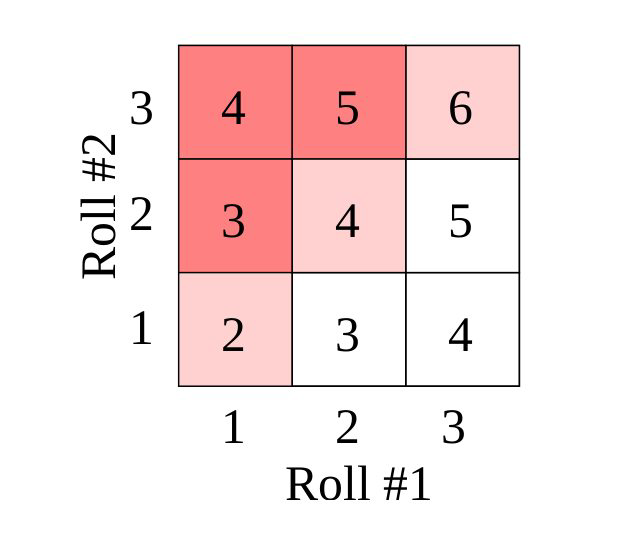
\includegraphics[width=2in]{Quizzes/fig1_4.png}\caption{Rolling two dice. In Bosons, one accepts only the rolls in the shaded squares, with equal probability 1/6. In Fermions, one accepts only the rolls in the darkly-shaded squares (not including the diagonal from lower left to upper right), with probability 1/3.}
    \label{fig:my_label}
\end{figure}


\begin{enumerate}
    \item Presume the dice are fair: each of the three numbers of dots shows up $1 / 3$ of the time. For a legal turn rolling a die twice in Bosons, what is the probability $\rho(4)$ of rolling a $4 ?$ Similarly, among the legal Fermion turns rolling two dice, what is the probability $\rho(4) ?$

\begin{Solution}
\begin{equation}
    \boxed{\rho_B(4) = \frac{2}{6}= \frac{1}{3}} \qquad \boxed{\rho_F(4) = \frac{1}{3}} 
\end{equation}
\end{Solution}

    \item For a legal turn rolling three `three-sided' dice in Fermions, what is the probability $\rho(6)$ of rolling a 6 ? (Hint: There is a Fermi exclusion princiTele: when playing Fermions, no two dice can have the same number of dots showing.) Electrons are fermions; no two electrons can be in exactly the same state. When rolling two dice in Bosons, there are six different legal turns $(11),(12),(13), \ldots,(33) ;$ half of them are doubles (both numbers equal), while for plain old Distinguishable turns only one-third would be doubles'; the probability of getting doubles is enhanced by 1.5 times in two-roll Bosons. When rolling three dice in Bosons, there are ten different legal turns $(111),(112),(113), \ldots,(333)$ When rolling $M$ dice each with $N$ sides in Bosons, one can show that there are
    $$
    \left(\begin{array}{c}
    N+M-1 \\
    M
    \end{array}\right)=\frac{(N+M-1) !}{M !(N-1) !}
    $$
    legal turns. 

\begin{Solution}
For this case, the only legal roll is (123). So, the probability is $\boxed{\rho_F(6)=1}$
\end{Solution}

    \item In a turn of three rolls, what is the factor by which the probability of getting triples in Bosons is enhanced over that in Distinguishable? In a turn of $M$ rolls, what is the enhancement factor for generating an M-tuple (all rolls having the same number of dots showing)? Notice that the states of the dice tend to cluster together in Bosons. Examples of real bosons clustering into the same state include Bose condensation (Section $7.6 .3 \text { ) and lasers (Exercise } 7.9)$

\begin{Solution}
\begin{equation}
    \rho_D(triple) = \frac{3}{27} \qquad \rho_B(triple) = \frac{3}{9}
\end{equation}
\begin{equation}
    \boxed{F = \frac{\rho_D}{\rho_B} = \frac{1}{3}}
\end{equation}
\end{Solution}
\end{enumerate}

\end{document}